% Diagrama das tarefas FreeRTOS no ESP32 — versão no estilo da Figura 7
% (mesma disposição da figura original; largura final 13,7 cm = 0.75\textwidth).
% Compilar com: pdflatex fluxograma_esp32_v2.tex
\documentclass[tikz,border=2pt]{standalone}
\usepackage[T1]{fontenc}
\usepackage[utf8]{inputenc}
\usepackage[scaled=0.95]{helvet}
\renewcommand{\familydefault}{\sfdefault}
\usepackage{amssymb}
\usetikzlibrary{shapes.geometric,arrows.meta,calc}

% Paleta da Figura 7
\definecolor{slate}{HTML}{3B4A5C}      % faixas de título
\definecolor{arrowc}{HTML}{4A6582}     % setas
\definecolor{contfill}{HTML}{F4F6FA}   % fundo dos contêineres
\definecolor{contdraw}{HTML}{A3AFC0}   % bordas
\definecolor{panel}{HTML}{E8EDF4}      % painéis cinza-azulados
\definecolor{lavfill}{HTML}{F1EEF6}    % lilás (decisões)
\definecolor{lavdraw}{HTML}{8E7CB0}
\definecolor{redfill}{HTML}{F9E9E5}    % ações de bloqueio
\definecolor{reddraw}{HTML}{B5544B}
\definecolor{grnfill}{HTML}{EEF3EA}    % início
\definecolor{grndraw}{HTML}{7FA06A}
\definecolor{grntext}{HTML}{4E7A3E}

\begin{document}
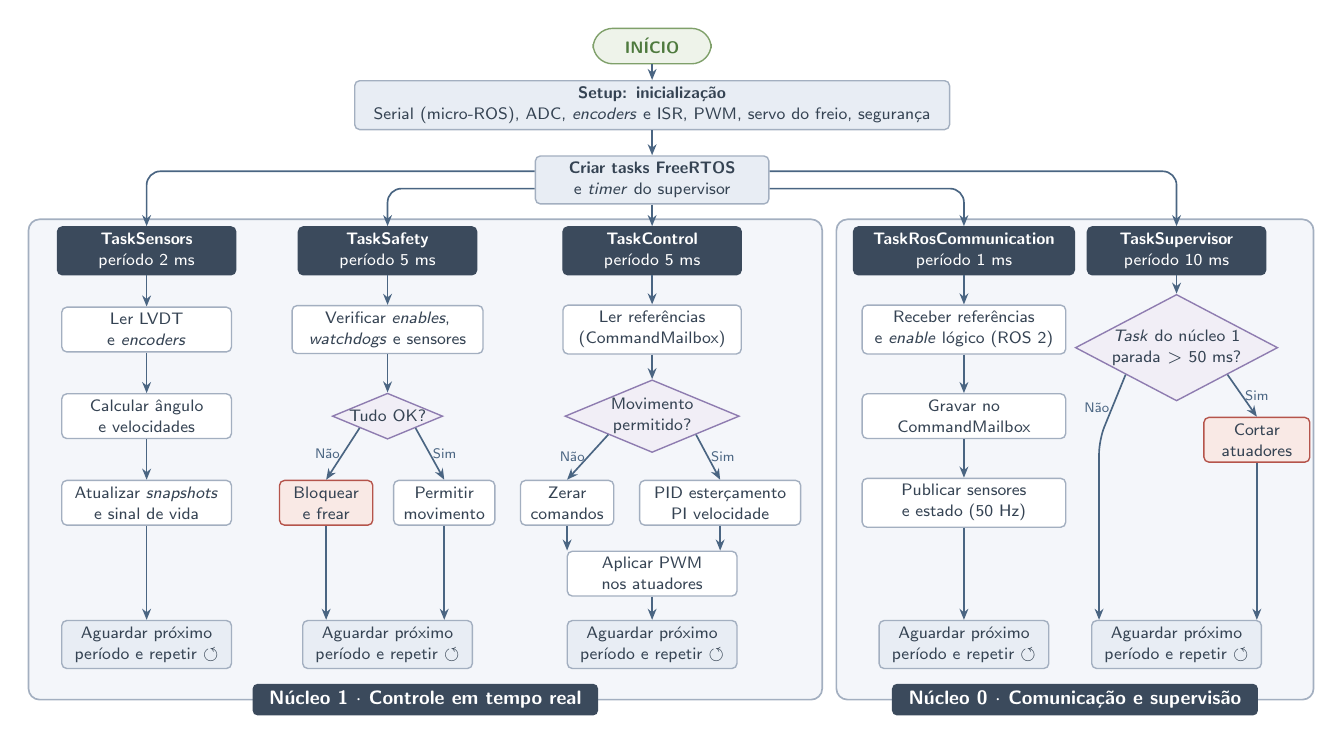
\begin{tikzpicture}[
    x=1.2cm,
    font=\fontsize{6.4}{7.6}\selectfont,
    >={Stealth[length=4pt,width=3.2pt]},
    line/.style={->,draw=arrowc,line width=0.6pt},
    base/.style={align=center,inner sep=2.2pt,minimum height=0.52cm,line width=0.5pt,text=slate!90!black},
    proc/.style={base,rectangle,rounded corners=1.8pt,fill=white,draw=contdraw},
    stop/.style={base,rectangle,rounded corners=1.8pt,fill=redfill,draw=reddraw},
    task/.style={base,rectangle,rounded corners=1.8pt,fill=slate,draw=slate,text=white,minimum height=0.5cm},
    dec/.style={base,diamond,aspect=2.4,inner sep=0.3pt,minimum height=0.5cm,fill=lavfill,draw=lavdraw},
    wait/.style={base,rectangle,rounded corners=1.8pt,fill=panel,draw=contdraw,minimum height=0.48cm},
    cont/.style={rounded corners=4pt,fill=contfill,draw=contdraw,line width=0.6pt},
    tab/.style={rectangle,rounded corners=1.8pt,fill=slate,text=white,font=\fontsize{6.6}{8}\selectfont\bfseries,inner xsep=6pt,inner ysep=2.6pt},
    lbl/.style={font=\fontsize{5.4}{6}\selectfont,text=arrowc,inner sep=0.8pt},
]

% ----------------------------------------------------------------- Contêineres
\draw[cont] (0.05,-2.45) rectangle (8.45,-8.55);
\draw[cont] (8.6,-2.45) rectangle (13.65,-8.55);
\node[tab] at (4.25,-8.55) {Núcleo 1 $\cdot$ Controle em tempo real};
\node[tab] at (11.125,-8.55) {Núcleo 0 $\cdot$ Comunicação e supervisão};

% ----------------------------------------------------------------- Inicialização
\node[base,rectangle,rounded corners=0.25cm,fill=grnfill,draw=grndraw,text=grntext,
      font=\fontsize{6.4}{7.5}\selectfont\bfseries,minimum width=1.5cm,minimum height=0.45cm] (ini) at (6.65,-0.25) {INÍCIO};
\node[proc,fill=panel,text width=7.4cm] (setup) at (6.65,-1.0)
    {\textbf{Setup: inicialização}\\Serial (micro-ROS), ADC, \textit{encoders} e ISR, PWM, servo do freio, segurança};
\node[proc,fill=panel,text width=2.81cm] (crt) at (6.65,-1.95)
    {\textbf{Criar \textit{tasks} FreeRTOS}\\e \textit{timer} do supervisor};
\draw[line] (ini) -- (setup);
\draw[line] (setup) -- (crt);

% ----------------------------------------------------------------- Linhas
\def\yh{-2.85}  % cabeçalhos das tasks
\def\ya{-3.85}
\def\yb{-4.95}
\def\yc{-6.05}
\def\yd{-6.95}
\def\yw{-7.85}  % aguardar

% ----------------------------------------------------------------- Núcleo 1
\node[task,text width=2.11cm] (s0) at (1.3,\yh) {\textbf{TaskSensors}\\período 2 ms};
\node[task,text width=2.11cm] (f0) at (3.85,\yh)  {\textbf{TaskSafety}\\período 5 ms};
\node[task,text width=2.11cm] (c0) at (6.65,\yh) {\textbf{TaskControl}\\período 5 ms};

\node[proc,text width=2.00cm] (s1) at (1.3,\ya) {Ler LVDT\\e \textit{encoders}};
\node[proc,text width=2.00cm] (s2) at (1.3,\yb) {Calcular ângulo\\e velocidades};
\node[proc,text width=2.00cm] (s3) at (1.3,\yc) {Atualizar \textit{snapshots}\\e sinal de vida};
\node[wait,text width=2.00cm] (s4) at (1.3,\yw) {Aguardar próximo\\período e repetir $\circlearrowleft$};

\node[proc,text width=2.27cm] (f1) at (3.85,\ya) {Verificar \textit{enables},\\\textit{watchdogs} e sensores};
\node[dec] (f2) at (3.85,\yb) {Tudo OK?};
\node[stop,text width=1.03cm] (f3n) at (3.2,\yc) {Bloquear\\e frear};
\node[proc,text width=1.13cm] (f3s) at (4.45,\yc) {Permitir\\movimento};
\node[wait,text width=2.00cm] (f4) at (3.85,\yw) {Aguardar próximo\\período e repetir $\circlearrowleft$};

\node[proc,text width=2.11cm] (c1) at (6.65,\ya) {Ler referências\\(CommandMailbox)};
\node[dec] (c2) at (6.65,\yb) {Movimento\\permitido?};
\node[proc,text width=1.03cm] (c3n) at (5.75,\yc) {Zerar\\comandos};
\node[proc,text width=1.89cm] (c3s) at (7.37,\yc) {\mbox{PID esterçamento}\\PI velocidade};
\node[proc,text width=2.00cm] (c4) at (6.65,\yd) {Aplicar PWM\\nos atuadores};
\node[wait,text width=2.00cm] (c5) at (6.65,\yw) {Aguardar próximo\\período e repetir $\circlearrowleft$};

% ----------------------------------------------------------------- Núcleo 0
\node[task,text width=2.65cm] (r0) at (9.95,\yh) {\textbf{TaskRosCommunication}\\período 1 ms};
\node[task,text width=2.11cm] (v0) at (12.2,\yh) {\textbf{TaskSupervisor}\\período 10 ms};

\node[proc,text width=2.43cm] (r1) at (9.95,\ya) {Receber referências\\e \textit{enable} lógico (ROS 2)};
\node[proc,text width=2.43cm] (r2) at (9.95,\yb) {Gravar no\\CommandMailbox};
\node[proc,text width=2.43cm] (r3) at (9.95,\yc) {Publicar sensores\\e estado (50 Hz)};
\node[wait,text width=2.00cm] (r4) at (9.95,\yw) {Aguardar próximo\\período e repetir $\circlearrowleft$};

\node[dec,aspect=1.9] (v1) at (12.2,-4.08) {\textit{Task} do núcleo 1\\parada $>$ 50 ms?};
\node[stop,text width=1.19cm] (v2) at (13.05,-5.25) {Cortar\\atuadores};
\node[wait,text width=2.00cm] (v3) at (12.2,\yw) {Aguardar próximo\\período e repetir $\circlearrowleft$};

% ----------------------------------------------------------------- Setas
% saídas laterais com curva de 90° arredondada
% (setas externas saem mais acima e as internas mais abaixo, para não se confundirem)
\draw[line,rounded corners=5pt] ($(crt.west)+(0,0.11)$) -| (s0.north);
\draw[line,rounded corners=5pt] ($(crt.west)+(0,-0.11)$) -| (f0.north);
\draw[line] (crt.south) -- (c0.north);
\draw[line,rounded corners=5pt] ($(crt.east)+(0,-0.11)$) -| (r0.north);
\draw[line,rounded corners=5pt] ($(crt.east)+(0,0.11)$) -| (v0.north);

\draw[line] (s0) -- (s1); \draw[line] (s1) -- (s2); \draw[line] (s2) -- (s3); \draw[line] (s3) -- (s4);

\draw[line] (f0) -- (f1); \draw[line] (f1) -- (f2);
\draw[line] (f2.south west) -- node[lbl,left] {Não} (f3n.north);
\draw[line] (f2.south east) -- node[lbl,right] {Sim} (f3s.north);
\draw[line] (f3n.south) -- (f3n.south |- f4.north);
\draw[line] (f3s.south) -- (f3s.south |- f4.north);

\draw[line] (c0) -- (c1); \draw[line] (c1) -- (c2);
\draw[line] (c2.south west) -- node[lbl,left] {Não} (c3n.north);
\draw[line] (c2.south east) -- node[lbl,right] {Sim} (c3s.north);
\draw[line] (c3n.south) -- (c3n.south |- c4.north);
\draw[line] (c3s.south) -- (c3s.south |- c4.north);
\draw[line] (c4) -- (c5);

\draw[line] (r0) -- (r1); \draw[line] (r1) -- (r2); \draw[line] (r2) -- (r3); \draw[line] (r3) -- (r4);

\draw[line] (v0) -- (v1);
\draw[line] (v1.south east) -- node[lbl,right] {Sim} (v2.north);
\coordinate (vn) at (11.38,-5.25);
\draw[line,rounded corners=5pt] (v1.south west) -- node[lbl,left] {Não} (vn) -- (vn |- v3.north);
\draw[line] (v2.south) -- (v2.south |- v3.north);

\end{tikzpicture}
\end{document}
